\subsection{Into}
Bei der Funkverbindung wurde auf das Radiohead-Paket\cite{rh} zurückgegriffen. Dieses Paket unterstützt viele gängige Sender/Empfänger-Kombinationen. Des weiteren ist anzumerken das hier die \grqq einfache\grqq  ASK\footnote{Amplitude Shift Keying/Amplitudenumtastung} Modulationsart verwendet wird. Dies wird durch das sogenannte On-Off Keying realisiert. \newline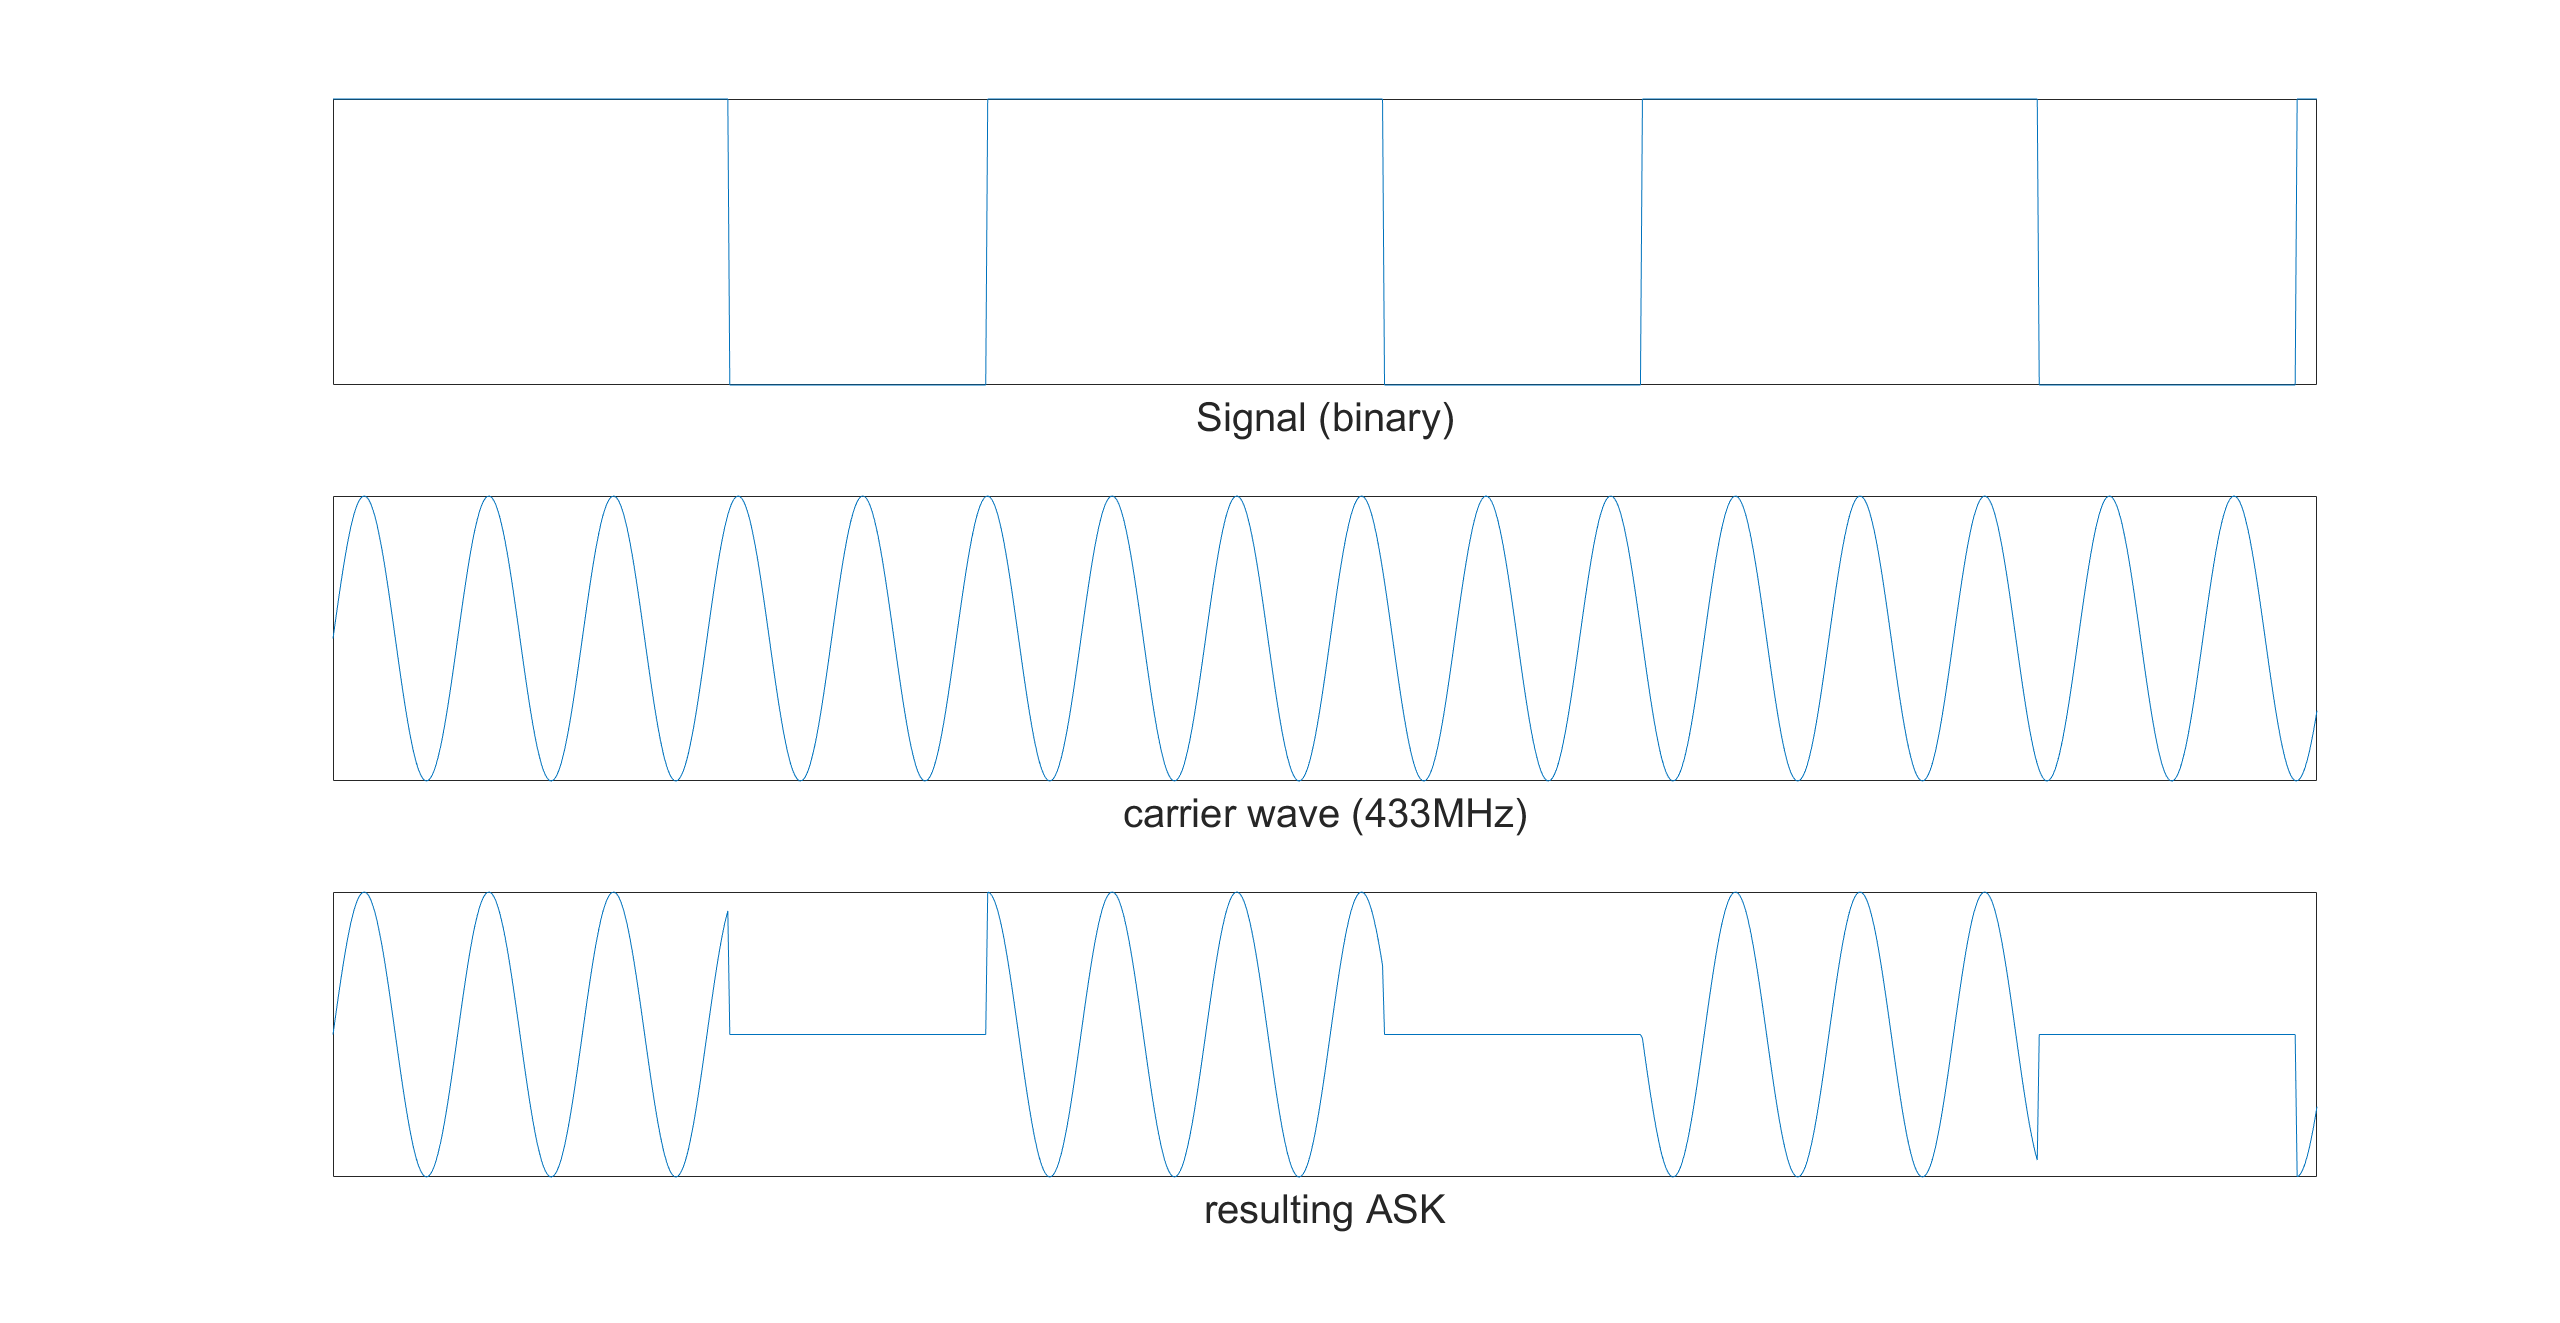
\includegraphics[width=\textwidth]{Hauptteil/sw/intro/ask.png}
Nachrichten des Radiohead-Pakets bestehen in unserer Anwendung aus unterschidlichen Teilen. Daraus ergibt sich eine stabile Funkverbindung.\\
%\newline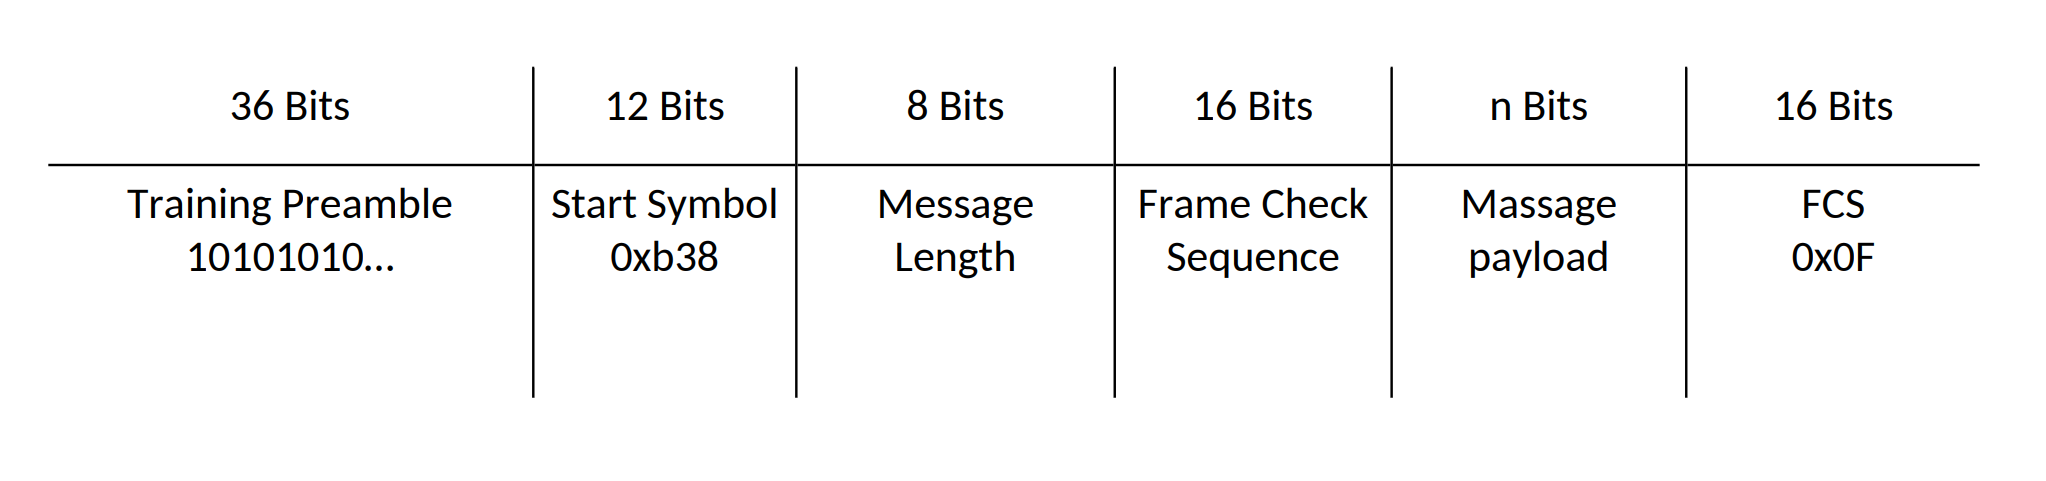
\includegraphics[width=\textwidth]{Hauptteil/sw/intro/packege.png}
\begin{tabularx}{\textwidth}{|X|X|l|X|X|X|}
\hline
 36 Bits & 12 Bits & 8 Bits & 16 Bits & n Bits & 16 Bits\\
\hline
Training Preamble for timing & Start Symbol 0xb38 & Nachrichtlänge & Frame Check Sequence & Nachrichten payload & FCS 0x0F\\
\hline
\end{tabularx}